% Requires running Bibtex

\documentclass[%
reprint,
amsmath,amssymb,
aps,
]{revtex4-2}

\usepackage{graphicx}% Include figure files
\usepackage{dcolumn}% Align table columns on decimal point
\usepackage{bm}% bold math
\usepackage{hyperref}% add hypertext capabilities
\usepackage[font=scriptsize,labelfont=bf, justification=justified]{caption}% change fontsize in captions
\usepackage{float}
\usepackage{booktabs}% cool table style
\hypersetup{
	colorlinks=true,       % false: boxed links; true: colored links
	linkcolor=black,        % color of internal links
	citecolor=black,        % color of links to bibliography
	filecolor=black,     % color of file links
	urlcolor=black         
}

\usepackage{bibspacing}
\setlength{\bibitemsep}{.5\baselineskip plus .05\baselineskip minus .05\baselineskip}


\begin{document}
	
	\preprint{APS/123-QED}
	
	\title{PHYC30170 Physics with Astronomy and Space Science Lab 1;\\Compton Scattering}
	
	\author{Daragh Hollman}
	\email{daragh.hollman@ucdconnect.ie}
	
	\date{\today}
	
	\begin{abstract}

	\end{abstract}

	\maketitle
	
	\section{Introduction}
	What is Compton scattering?\\
	Applications: Inelastic photon scattering: Effects and applications in biomedical science and industry\cite{harding}\\
	Why it is important to understand\\
	
	Compton scattering is the interaction in the collision of a gamma ray with a free electron \cite{manual1}.
	
	\section{Energy and Cross-Section Determination}
	
		\subsection{Theory}
			

			\begin{figure}
				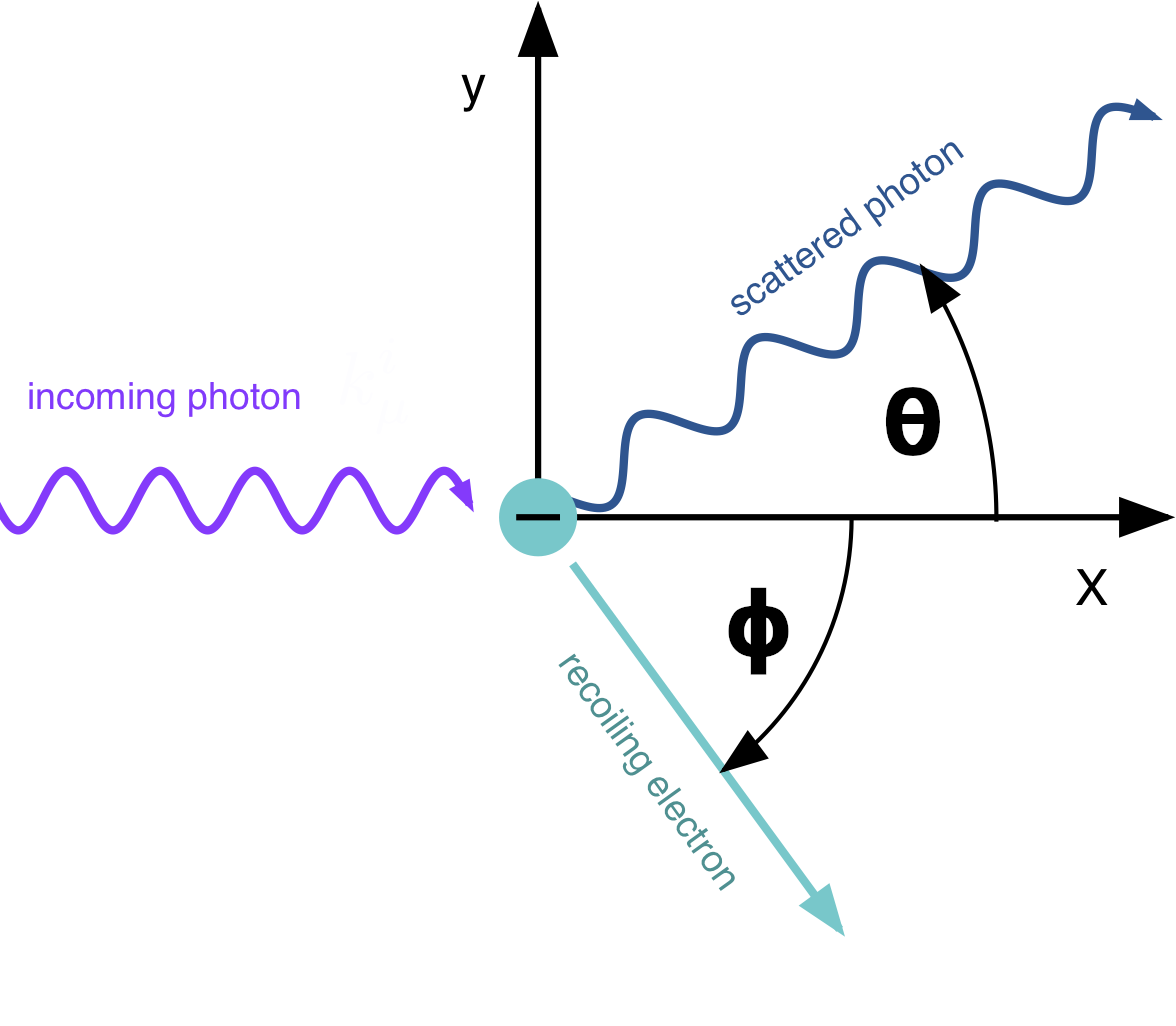
\includegraphics[width=0.7\columnwidth]{compton_scattering.png}
				\caption{\label{fig:diagram}A diagram of the Compton scattering interaction. A photon is scattered off an electron with a transfer of energy.}
			\end{figure}
		
		\subsection{Methodology}
		
		\subsection{Results and Analysis}
		
	\section{Relativity and the Electron Rest Mass}
	
		\subsection{Theory}
		
		\subsection{Methodology}
		
		\subsection{Results and Analysis}


	\section{Conclusion}

		
		
	\clearpage
	\bibliography{comptonscattering}% Produces the bibliography via BibTeX.

		
\end{document}

